\clearpage

\section{Pythagoran kolmio}

Peikko Pythagora työskentelee Draculan linnan työmaalla. Hänen tehtävänään on tukea rakennustelineet. Jotta telineistä tulisi tukevat, täytyy niiden kulmiin asentaa suorakulmaiset kolmiot. Pythagora on kuitenkin unohtanut suorakulmansa kotiin. Hän on mitannut $8 \text{cm}$, $15 \text{cm}$ ja $18 \text{cm}$ palat. Saako Pythagora näistä paloista rakennettua suorakulmaisen kolmion?

\begin{figure}[h]
    \begin{center}
    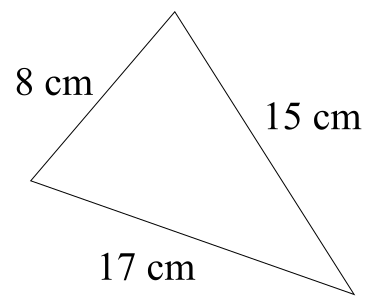
\includegraphics[width=0.5\linewidth]{kuvat/pythagoran_kolmio}
    \end{center}
\end{figure}